% Study 2, the results, from the inference, integrity and post-hoc files of the two runs under reports/ and
% the post-hoc dynamic-occurrence directory. Input from paper.tex; every number traces to sources.md and is
% asserted by check_numbers.py. Macros are provided in case the file is compiled before paper.tex defines
% them.
\providecommand{\lm}{\texttt{local\_mean\_28}}
\providecommand{\aets}{\texttt{autoets\_weekly}}
\providecommand{\qs}{QScore9}
\providecommand{\hc}{\texttt{hurdle\_count\_28}}

\section{Study 2: results}
\label{sec:s2results}

Tables~\ref{tab:s2ext} and~\ref{tab:s2syn} give the eighteen external and the six synthetic comparisons
with the columns of Tables~\ref{tab:lm} and~\ref{tab:ae}; differences are model variant minus reference, so
negative favors the variant, and every external mean is carried by one series (Section~\ref{sec:s2panel}).
Twelve of the eighteen external tests and five of the six synthetic tests reject at $q = 0.05$ after one
adjustment per family; of the twelve, ten reject for the model variant and two against it, and all five
synthetic rejections are against the hurdle variant. Figure~\ref{fig:s2npm} shows the 209 paired differences
behind each external row. Each run ran once on 2026-10-15 with no failed window, and every one of the 20,064
npm and 55,080 synthetic scores was recomputed from the saved forecasts with no disagreement
(Appendix~\ref{app:s2repro}).

\begin{table}[t]
\centering\footnotesize\setlength{\tabcolsep}{3.5pt}
\caption{The eighteen declared external comparisons on the npm panel. Differences are model variant minus
reference \qs{}, averaged over three origins within series and then over 209 series; negative favors the
variant. The contrast names the pair: the model's hurdle against its completed control, the hurdle against
\hc{}, or the raw deciles against \lm{} (the full tuples are in Appendix Table~\ref{tab:s2family}). The
interval is the pointwise 95 percent percentile interval from 20,000 series-cluster bootstrap replicates.
``Lower / tied / higher'' counts the series (of 209) where the variant's score is below, equal to or above
the reference's. $p$ is the Benjamini-Hochberg adjusted two-sided Wilcoxon signed-rank $p$-value over the
18 tests. Every mean in this table is carried by the series \texttt{aggregate-error}
(Section~\ref{sec:s2panel}); the medians, counts and tests are rank-based and describe the typical series.}
\label{tab:s2ext}
\begin{tabular}{lllrrcrcl}
\toprule
ID & Model & Contrast & $h$ & Mean & 95\% interval & Median & Lower / tied / higher & Adjusted $p$ \\
\midrule
E01 & Chronos-2 & hurdle vs completed & 7 & 152 & [0.1846, 455.2] & -0.01376 & 121 / 2 / 86 & 0.203 \\
E02 & Chronos-2 & hurdle vs count hurdle & 7 & -5,090 & [-15,175, -31.08] & -0.01587 & 129 / 12 / 68 & $3.72 \times 10^{-11}$ \\
E03 & Chronos-2 & raw vs local mean & 7 & -2,884 & [-8,601, -17.33] & 0.007856 & 92 / 0 / 117 & 0.596 \\
E04 & Chronos-2 & hurdle vs completed & 30 & 90.24 & [0.2273, 269.7] & -0.0002469 & 105 / 2 / 102 & 0.449 \\
E05 & Chronos-2 & hurdle vs count hurdle & 30 & -6,563 & [-19,596, -30.03] & -0.06173 & 150 / 9 / 50 & $7.06 \times 10^{-21}$ \\
E06 & Chronos-2 & raw vs local mean & 30 & -4,734 & [-14,149, -15.84] & -0.002372 & 112 / 0 / 97 & 0.0119 \\
E07 & TimesFM 3 & hurdle vs completed & 7 & 176.9 & [0.2669, 529.4] & 0.001058 & 94 / 8 / 107 & 0.236 \\
E08 & TimesFM 3 & hurdle vs count hurdle & 7 & -5,416 & [-16,153, -31.67] & -0.007407 & 116 / 18 / 75 & $3.61 \times 10^{-8}$ \\
E09 & TimesFM 3 & raw vs local mean & 7 & -3,235 & [-9,650, -18.24] & -0.002297 & 112 / 1 / 96 & 0.0438 \\
E10 & TimesFM 3 & hurdle vs completed & 30 & 128.5 & [0.5058, 383.8] & 0.00321 & 81 / 8 / 120 & 0.00215 \\
E11 & TimesFM 3 & hurdle vs count hurdle & 30 & -6,792 & [-20,280, -31.3] & -0.0716 & 161 / 17 / 31 & $3.19 \times 10^{-25}$ \\
E12 & TimesFM 3 & raw vs local mean & 30 & -5,001 & [-14,947, -16.86] & -0.005016 & 125 / 1 / 83 & $3.82 \times 10^{-5}$ \\
E13 & TimesFM 2.5 & hurdle vs completed & 7 & 253.9 & [0.5046, 759.9] & -0.002116 & 109 / 3 / 97 & 0.628 \\
E14 & TimesFM 2.5 & hurdle vs count hurdle & 7 & -5,847 & [-17,446, -30.83] & -0.006349 & 115 / 7 / 87 & $2.66 \times 10^{-5}$ \\
E15 & TimesFM 2.5 & raw vs local mean & 7 & -3,743 & [-11,179, -17.41] & 0.01696 & 84 / 1 / 124 & 0.746 \\
E16 & TimesFM 2.5 & hurdle vs completed & 30 & 110.3 & [0.6883, 328.7] & 0.0009877 & 101 / 1 / 107 & 0.0276 \\
E17 & TimesFM 2.5 & hurdle vs count hurdle & 30 & -6,918 & [-20,665, -29.9] & -0.06938 & 160 / 9 / 40 & $1.77 \times 10^{-23}$ \\
E18 & TimesFM 2.5 & raw vs local mean & 30 & -5,109 & [-15,279, -15.49] & -0.003695 & 113 / 1 / 95 & 0.00204 \\
\bottomrule
\end{tabular}
\end{table}

\begin{table}[t]
\centering\footnotesize\setlength{\tabcolsep}{3.5pt}
\caption{The six declared synthetic comparisons at horizon 30. Differences are model variant minus reference
\qs{}, averaged over three origins within each replicate and cell, then over the 18 cells with equal weight,
so that each of the 30 replicate blocks carries one paired difference; negative favors the variant. The
interval is the pointwise 95 percent percentile interval from 20,000 replicate-block bootstrap replicates.
``Lower / tied / higher'' counts the blocks (of 30) where the variant's score is below, equal to or above
the reference's. $p$ is the Benjamini-Hochberg adjusted two-sided Wilcoxon signed-rank $p$-value over the
6 tests.}
\label{tab:s2syn}
\begin{tabular}{lllrrcrcl}
\toprule
ID & Model & Contrast & $h$ & Mean & 95\% interval & Median & Lower / tied / higher & Adjusted $p$ \\
\midrule
S01 & Chronos-2 & hurdle vs completed & 30 & 0.08599 & [0.03836, 0.1401] & 0.05554 & 6 / 0 / 24 & 0.00415 \\
S02 & Chronos-2 & hurdle vs count hurdle & 30 & 0.05211 & [0.01686, 0.09227] & 0.04737 & 9 / 0 / 21 & 0.0111 \\
S03 & TimesFM 3 & hurdle vs completed & 30 & 0.08662 & [0.03837, 0.1429] & 0.06144 & 6 / 0 / 24 & 0.00676 \\
S04 & TimesFM 3 & hurdle vs count hurdle & 30 & 0.0215 & [-0.006569, 0.04947] & 0.03119 & 11 / 0 / 19 & 0.12 \\
S05 & TimesFM 2.5 & hurdle vs completed & 30 & 0.08769 & [0.04316, 0.1382] & 0.06743 & 5 / 0 / 25 & 0.00415 \\
S06 & TimesFM 2.5 & hurdle vs count hurdle & 30 & 0.06109 & [0.02299, 0.09881] & 0.06027 & 9 / 0 / 21 & 0.00798 \\
\bottomrule
\end{tabular}
\end{table}

\paragraph{Three zero days in the npm targets.} After the run was scored, the saved targets were found to
read 0 for every one of the 209 series on 2026-07-12 and 2026-08-14, and 0 for \texttt{aggregate-error}
alone on 2026-06-25, between days of millions (Appendix~\ref{app:s2tables}). The registered completeness
rule, fixed before any target was seen, does not test for a source-wide zero, so the three days were scored
as served; each falls in one horizon-30 block and in no horizon-7 block. npm's own records report no outage
or backfill for them, and a public thread records two earlier episodes in which whole days read 0 for nearly
every package and were later restored \citep{npm-community-150808}. The dated addition of 2026-10-16 to the
protocol, item 6, made after the scores were seen, keeps the registered analysis of the data as served as
the confirmatory result for E01 to E18 and asks that a post-hoc sensitivity which removes the days be
reported beside it; that sensitivity, computed at 03:21 UTC on 2026-10-16 before the addition was written
at 03:28 UTC and committed with it, is at the end of this section.

\paragraph{Occurrence replaced, positive law kept (E01, E04, E07, E10, E13, E16; S01, S03, S05).} Against
its own completed control, the hurdle variant's mean difference is positive, favoring the control, in all six
external cells, from 90.24 to 253.9 (carried by \texttt{aggregate-error}), with every interval above zero;
the medians lie within 0.014 of zero, three below it and three above; the hurdle scores lower on 81 to 121
of the 209 series; and the signed-rank test rejects after adjustment in two of the six cells, TimesFM 3 and
TimesFM 2.5 at horizon 30 (E10, with the hurdle higher on 120 of 209 series and adjusted $p$ 0.00215; E16,
higher on 107, adjusted $p$ 0.0276), on the side of the control. The other four are not rejected, with
adjusted $p$ from 0.203 to 0.628; not rejecting is not equivalence. No test favors the substitution at
$q = 0.05$, but in E01 the typical series leans to the hurdle, lower on 121 of 209 series with a median of
-0.01376 and the larger signed-rank sum on its side, and in E04 and E13 the medians and counts lean to the
hurdle while the rank sums lean to the control. On the grid the hurdle's mean difference against its own
control favors the control for all three models, from 0.08599 to 0.08769, with every interval above zero;
the hurdle scores lower on 5 or 6 of the 30 replicate blocks; and all three tests reject, with adjusted $p$
from 0.00415 to 0.00676, against the hurdle. Table~\ref{tab:s2parts} splits each hurdle-minus-control
difference into the three exact accounting parts of Section~6: on the mean, in every one of the nine cells
the substitution lowers the zero-day loss and the positive-day overprediction loss and raises the
positive-day underprediction loss by more than both, so the net sign is the control's. On the mean the trade
goes the same way on both studies; the typical npm series does not follow it, since the median series'
zero-day difference is positive, against the hurdle, in all six cells (0.003 to 0.036).

\begin{table}[t]
\centering\small
\caption{The hurdle-minus-control difference (E01, E04, E07, E10, E13, E16 on npm; S01, S03, S05 on the
grid) and its three exact accounting parts, each divided by the full horizon: the loss on zero target days,
the loss on positive days from quantiles above the target (overprediction) and from quantiles below it
(underprediction). Equal-series and equal-block means; the parts sum to the total. Negative favors the
hurdle. The npm parts are unscaled and \texttt{aggregate-error} dominates them.}
\label{tab:s2parts}
\begin{tabular}{llrrrrr}
\toprule
Study & Model & $h$ & Total & Zero days & Positive, overprediction & Positive, underprediction \\
\midrule
npm & Chronos-2 & 7 & 152 & -0.3176 & -161.7 & 314 \\
npm & TimesFM 3 & 7 & 176.9 & -0.3701 & -149.5 & 326.8 \\
npm & TimesFM 2.5 & 7 & 253.9 & -0.3425 & -91.81 & 346 \\
npm & Chronos-2 & 30 & 90.24 & -63.79 & -146.1 & 300.1 \\
npm & TimesFM 3 & 30 & 128.5 & -66.08 & -112.9 & 307.5 \\
npm & TimesFM 2.5 & 30 & 110.3 & -67.09 & -131.9 & 309.4 \\
synthetic & Chronos-2 & 30 & 0.08599 & -0.1752 & -0.03194 & 0.2931 \\
synthetic & TimesFM 3 & 30 & 0.08662 & -0.172 & -0.0282 & 0.2868 \\
synthetic & TimesFM 2.5 & 30 & 0.08769 & -0.2293 & -0.03873 & 0.3557 \\
\bottomrule
\end{tabular}
\end{table}

\paragraph{The regime reading, from the declared secondary strata.} The confirmatory families pool 209
equal-weight series and 18 equal-weight cells, so they speak for whatever dominates the pool: on npm the
dense stratum, whose unscaled losses are the largest, and on the grid the cells with $z = 0.2$ and
$\mu_{+} = 25$. The declared secondary stratum tables (Appendix Table~\ref{tab:s2strata}) read
differently by regime: against its completed control the hurdle variant scores lower on 81, 60 and 66 of
the 100 sparse series at horizon 7, for Chronos-2, TimesFM 3 and TimesFM 2.5, and on 58, 45 and 54 of
them at horizon 30, while on the dense series it scores lower on 32 to 43 of 100 in every cell, and on
the grid it beats its control in 4 to 6 of 30 replicate blocks at $z = 0.2$ against 21 to 26 at
$z = 0.95$. A post-hoc signed-rank test within each stratum rejects for all three sparse-stratum
contrasts at horizon 7 and for none at horizon 30, and the dense result has a mechanical cause in the
zero mass the Jeffreys rule forces onto a series with no recent zero (Appendix~\ref{app:s2tables},
Tables~\ref{tab:s2regime} and~\ref{tab:s2cells}). So the substitution hurts the typical dense series
and the short-memory cells, helps the typical sparse series at horizon 7, and is null at 30 days. This
was the paper's central descriptive finding, a reading of declared secondary tables and not a
confirmatory result; Study 3 registered it as a per-stratum family and tested it on a second domain
(Section~\ref{sec:s3results}).

\paragraph{The model's positive law against a fixed count hurdle (E02, E05, E08, E11, E14, E17; S02, S04,
S06).} Against \hc{}, which shares the hurdle variant's occurrence probability and differs only in its
shifted-Poisson positive law, all six external tests reject in favor of the variant, with adjusted $p$ from
$2.66 \times 10^{-5}$ to $3.19 \times 10^{-25}$: the mean difference favors the variant in every cell, from
-5,090 to -6,918 (carried by \texttt{aggregate-error}), with every interval below zero; the medians are
negative, from -0.006349 to -0.0716; and the variant scores lower on 115 to 161 of the 209 series. The
occurrence Brier difference is exactly zero for every series in these six rows, so the gain is in the
positive law. By stratum the variant is lower than \hc{} on 80 to 94 of the 100 dense series and on 29 to
63 of the 100 sparse ones: a shifted Poisson cannot fit a series with thousands of downloads a day, so on
dense series this is a win over a comparator that cannot win. Against the registered secondary
\texttt{hurdle\_empirical\_28}, which shares the occurrence rule and uses the empirical positive law, a
post-hoc reading of the saved per-series scores (Appendix Table~\ref{tab:s2empirical}) narrows the claim:
the completed control is lower than the empirical hurdle on 120 to 140 of 209 series at horizon 30 for all
three models but at horizon 7 on only 88 and 90 of 209 for Chronos-2 and TimesFM 2.5 (117 for TimesFM 3),
and the foundation-model hurdle is lower on 63 to 72 of the 100 dense series and on 33 to 57 of the 100
sparse. On the grid the registered contrast goes the other way or is not rejected: the Chronos-2 and TimesFM
2.5 hurdles score higher than the count hurdle, by 0.05211 and 0.06109 (adjusted $p$ 0.0111 and 0.00798,
lower on 9 of 30 blocks each), and the TimesFM 3 hurdle differs by 0.0215 with an interval that includes
zero (adjusted $p$ 0.12, lower on 11 of 30), leaning the same way without rejection. So the model's
completed size forecast beats a shifted Poisson where the Poisson is misspecified and not where it is the
generator's own law; against an empirical positive law its advantage holds at 30 days and on dense series,
not in general.

\paragraph{The dynamic count.} The registered \texttt{dynamic\_count} baseline, which carries no foundation
model, is the best non-oracle forecaster on the grid: its mean \qs{} at horizon 30 is 1.721 against 1.754 to
1.792 for the three completed models, 1.819 for \hc{} and 1.648 for the oracle (Appendix
Table~\ref{tab:s2synscores}), and by replicate block it is lower than the completed Chronos-2, TimesFM 3 and
TimesFM 2.5 in 21, 18 and 24 of 30 blocks and lower than \hc{} and \lm{} in 26 of 30. On npm it loses: the
completed models are lower on 108 to 146 of 209 series, and its mean \qs{} is 10,948 and 11,471 at the two
horizons against 3,641 to 4,500 for the completed models (Appendix Table~\ref{tab:s2scores}). These are
readings of declared secondary tables and saved scores, with no test.

\paragraph{The raw deciles against the local mean (E03, E06, E09, E12, E15, E18).} Four of the six tests
reject in favor of the model, Chronos-2 at horizon 30 (E06), TimesFM 3 at both horizons (E09, E12) and
TimesFM 2.5 at horizon 30 (E18); Chronos-2 and TimesFM 2.5 at horizon 7 (E03, E15) are not rejected, with
adjusted $p$ 0.596 and 0.746. The mean difference favors the model in all six cells, from -2,884 to -5,109
(carried by \texttt{aggregate-error}), with every interval below zero, and the models score lower on 84 to
125 of the 209 series. The medians favor the reference at horizon 7 for Chronos-2 and TimesFM 2.5 (0.007856
and 0.01696) and the model in the other four cells (-0.002297 to -0.005016). At horizon 30 the typical npm
series favors the frozen models, rejecting on the model's side in four cells, with the rank sums leaning that
way in the other two while their medians favor the reference; in Study 1 the rank test favored the reference
in all nine cells.

\paragraph{The one series behind every npm mean.} In each of the eighteen rows of Table~\ref{tab:s2ext}
the series whose omission moves the mean most is \texttt{aggregate-error}, and its paired difference has the
sign of the row's mean in every row. Without it the six hurdle-against-control means fall from 90.24 to
253.9 to 0.6334 to 1.599, and in the twelve rows against \hc{} and \lm{} the five largest positive gains
hold 0.995 to 0.998 of all positive gain. The context-scaled \qs{}, the registered scale-free secondary,
favors the hurdle over its control at horizon 7 for all three models, with every interval below zero, and
includes zero at horizon 30, agreeing with the medians where the unscaled mean differs (Appendix
Table~\ref{tab:s2scaled}). The Brier score, the oracle, which no forecaster scores below in 17 of the 18
cells, and the per-cell differences are in Appendix~\ref{app:s2tables}.

\begin{figure}[t]
\centering
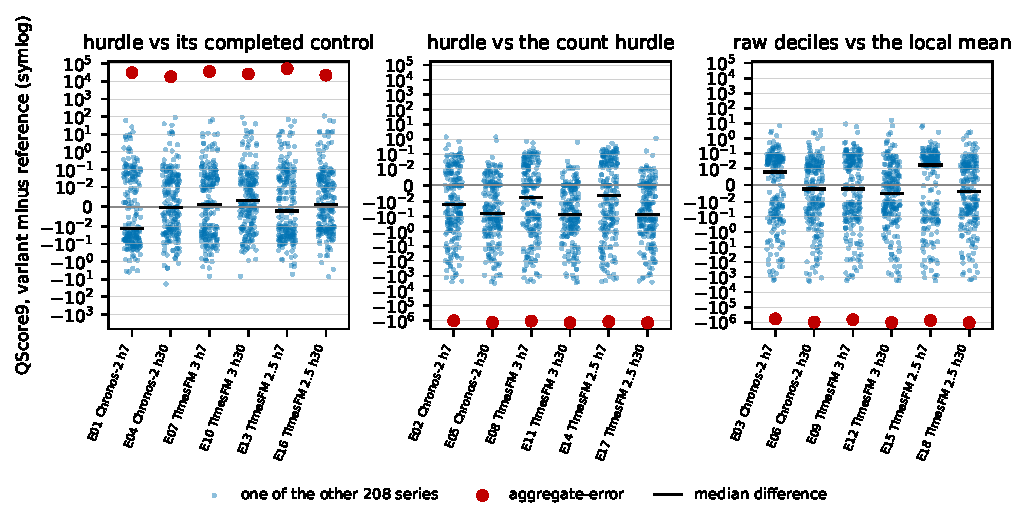
\includegraphics[width=\textwidth]{fig-s2-npm-paired-differences}
\caption{The eighteen external comparisons, series by series. Each point is one of the 209 series' paired
difference (variant minus reference \qs{}, three origins averaged) on a symmetric log scale, grouped by
contrast; the filled red marker is \texttt{aggregate-error}, and the short bar is the median. The mean of
each row, in Table~\ref{tab:s2ext}, is the red marker's value divided by 209 plus a remainder of a different
order.}
\label{fig:s2npm}
\end{figure}

\paragraph{Post-hoc: the family without the three zero days.} This paragraph is post-hoc. It was computed
on 2026-10-16 from the saved npm forecasts, after the registered scores were seen and before item 6 of the
dated addition of 2026-10-16 was written; the addition keeps the registered analysis as the default, so no
confirmatory result depends on the order. Each removed day is dropped from the one horizon-30 block that
holds it, the block is re-scored over its remaining 29 days, and the registered aggregation, test, seeded
bootstrap and one adjustment run unchanged (Appendix Table~\ref{tab:s2sens}). Without all three days, which
re-scores 10,032 forecasts, none of the eighteen conclusions changes: no row changes the side with the
larger signed-rank sum, the sign of its mean or its rejection. Without the two panel-wide days only, which
re-scores 6,688 forecasts, one conclusion changes: E06, Chronos-2's raw deciles against \lm{} at horizon 30,
no longer rejects, with adjusted $p$ 0.0599 and raw $p$ 0.0399 against 0.0119 and 0.00663 registered; it
still favors the model by rank sum, with the model lower on 110 of 209 series. Without the three days the
hurdle-against-control means at horizon 30 grow, E04 from 90.24 to 159.3, E10 from 128.5 to 201.2 and E16
from 110.3 to 183.4, and those means belong to \texttt{aggregate-error}. The mechanism answer does not
depend on the three days.

\paragraph{Post-hoc: the model's positive law with the dynamic count's occurrence.} This paragraph is
post-hoc. It was computed on 2026-10-16 from the saved forecasts of both runs, after the registered
scores were seen, with no registered status; it adds no test to E01 to E18 or S01 to S06 and replaces
nothing in them, and no model was run. The wrapper is the registered hurdle with the Jeffreys $p$
replaced by the occurrence probability of \texttt{dynamic\_count}'s saved law for the same day, the
discounted Beta-Bernoulli with discount 0.98, with $G_+$ the model's saved completed positive law exactly
as the registered hurdle uses it; it is compared with the model's completed control, its registered
hurdle, \texttt{dynamic\_count} and \hc{} in two post-hoc families, 24 tests on npm and 12 on the grid,
each with the registered settings and its own adjustment at $q = 0.05$ (Appendix
Tables~\ref{tab:s2dyn} and~\ref{tab:s2dynrest}). The dynamic occurrence shrinks the loss and removes
four of the five rejections against the substitution, and it still never beats the model's own zero mass
at $q = 0.05$: against the completed control no npm row and one grid row reject, with every mean
difference still positive; against the registered fixed-occurrence hurdle the wrapper rejects in its
favor at horizon 30 on npm and on the grid; and on the grid it has the lowest zero-day part of every
forecaster while its positive-day underprediction part stays above the completed controls' and
\texttt{dynamic\_count}'s, so with the occurrence held equal the remaining loss is the positive law
(Appendix~\ref{app:s2tables}). Study 3 carries this occurrence into a registered family
(Section~\ref{sec:s3design}).

\paragraph{Read together.} Replacing a frozen model's own zero mass with the 28-day context-only occurrence
probability, keeping the model's completed positive law, does not lower \qs{} on the pooled families, which
speak for the dense regime; by stratum the typical sparse series at horizon 7 favors the substitution, the
typical dense series favors the control, and at 30 days the strata are null. A dynamic occurrence estimate
narrows the gap and does not close it. The model's positive law beats a shifted-Poisson count hurdle in all
six npm cells and loses or is not rejected on the grid; against an empirical positive law its advantage holds
at 30 days and on dense series. The registered dynamic count beats every foundation model on the grid and
loses to them on npm. The raw deciles beat the local mean on the npm mean in every cell and on the rank test
at horizon 30 for all three models. Null, adverse, mixed and
imprecise outcomes are reported with the same care as a positive one.
